% !TEX option = --shell-escape
% !TEX program = xelatex
\documentclass[fontset=fandol]{ctexart}

\setmainfont{Linux Libertine O}
\setsansfont{Linux Biolinum O}

\usepackage[dvipsnames]{xcolor}
\usepackage{pgfornament-han}
\usetikzlibrary{chains}
\usetikzlibrary{calc}
\usetikzlibrary{decorations}
\usetikzlibrary{decorations.text,decorations.markings}

\usepackage{cncolours}

\usepackage{geometry}
\geometry{hmargin=1in,vmargin=0.8in,headheight=10pt}

\usepackage{tcolorbox}
\tcbuselibrary{skins,raster}


%%%%%% 这段代码可以忽视,只是 --shell-escape 时调用 minted 不然就用 listings
\ifnum\shellescape=1
  \tcbuselibrary{minted}
  \setminted{breaksymbolleft={},breakindent=\ccwd}
  \newminted{latex}{}
  \newmintinline{latex}{}
\else
  \tcbuselibrary{listings}
  \newcommand{\latexinline}[1]{\lstinline|#1|}
  \lstnewenvironment{latexcode}{\lstset{language={[LaTeX]TeX}}}{}
  \lstset{basicstyle=\ttfamily}
\fi
%%%%%%%%


\tcbset{fonttitle=\kaishu\large\bfseries,colback=铅白!60!white,colbacktitle=绀青,coltitle=精白,colframe=墨灰}

\makeatletter
\newcommand{\getpgfornamenthanDim}[1]{%
 {\@pgfornamenthanDim{#1}宽:\@pgfornamentX\\高:\@pgfornamentY}%
}
\makeatother

\usepackage{fancyhdr}
\fancyhf{}
\renewcommand{\headrule}{}

\fancyhead[L]{%
\newbox{\fortyseven}
\savebox{\fortyseven}{\pgfornamenthan[scale=0.2,color=鸭卵青]{47}}
\tikzset{every node/.append style={inner sep=0pt,鸭卵青}}
\begin{tikzpicture}[overlay,remember picture]
\node[anchor=north west,shift={(14.5pt,-14.5pt)}] at (current page.north west)
  (nw) {\pgfornamenthan[scale=0.2]{25}};
\node[anchor=north east,shift={(-14.5pt,-14.5pt)}] at (current page.north east)
  (ne) {\pgfornamenthan[scale=0.2,symmetry=v]{25}};
\node[anchor=south west,shift={(14.5pt,14.5pt)}] at (current page.south west)
  (sw) {\pgfornamenthan[scale=0.2,symmetry=h]{25}};
\node[anchor=south east,shift={(-14.5pt,14.5pt)}] at (current page.south east)
  (se) {\pgfornamenthan[scale=0.2,symmetry=c]{25}};
%
\begin{scope}[start chain,node distance=0pt]
\node[anchor=north west,on chain] at (nw.north east) {\usebox{\fortyseven}};
\foreach \i in {1,...,15} {
  \node[on chain]{\usebox{\fortyseven}};
}
\end{scope}
%
\begin{scope}[start chain,node distance=0pt]
\node[anchor=south west,on chain] at (sw.south east) {\usebox{\fortyseven}};
\foreach \i in {1,...,6} \node[on chain]{\usebox{\fortyseven}};
\end{scope}
%
\begin{scope}[start chain=going left,node distance=0pt]
\node[anchor=south east,on chain] at (se.south west) {\usebox{\fortyseven}};
\foreach \i in {1,...,6} \node[on chain]{\usebox{\fortyseven}};
\end{scope}
%
% 垂直的话 chains 比较不好控制,我懒得折腾了,直接用 \foreach。
% 自己算一下, (47) 长度 155. 那么 scale = 0.2 的话……
\foreach \i in {0,...,21}
  \node[anchor=south west,rotate=-90,shift={($\i*(31bp,0)$)}] at (nw.south west)
    {\usebox{\fortyseven}};
%
\foreach \i in {0,...,21}
  \node[anchor=south east,rotate=90,shift={($\i*(-31bp,0)$)}] at (ne.south east)
    {\usebox{\fortyseven}};
%
%% 严格来说应该放在 \fancyfoot 吧,算了一样啦
\node[yshift=32pt,铜绿] at (current page.south) {\pgfornamenthan[scale=0.1]{51}};
\node[yshift=32pt,text=black] at (current page.south) {\large\thepage};
%
\end{tikzpicture}
}

\pagestyle{fancy}
\fancypagestyle{plain}{\pagestyle{fancy}}

\usepackage[hidelinks]{hyperref}

\title{汉风图纹 \texttt{pgfornament-han} v0.32}
\author{林莲枝、张晨南}
\date{v0.32 2018/04/09\\\url{https://github.com/liantze/pgfornament-han}}

\begin{document}

\maketitle

\begin{abstract}
利用 \texttt{pgfornament} 宏包可以在 \LaTeX{} 文件里便捷地画出十分典雅漂亮的、欧式风格的花纹。(详情请自行访问 \url{http://ctan.org/pkg/pgfornament})
 \texttt{pgfornament-han} 宏包的用意,正是为了尝试用 \texttt{pgfornament} 的已有机制,提供一些汉风的传统图纹。所有图纹均由\emph{张晨南}以 CAD 程式定稿、TikZ 绘制,再由\emph{林莲枝}转为适合 \texttt{pgfornament} 机制使用的宏包代码。
\end{abstract}

\part{基本用法}

\texttt{n} 为图纹编号的话,最简单的用法是 \latexinline{\pgfornamenthan[color=red,width=1.5cm]{n}}。
也可以用 \texttt{height} 或者 \texttt{scale} 设定大小。注意图纹比例是不变的,因此只有最后给出的选项有效。此外 \texttt{symmetry} 参数可以实现3种镜像,\texttt{v} (垂直)、\texttt{h}(水平)、\texttt{c}(中心=垂直+水平镜像),画边框的四个角点时很好用。其它TikZ 参数的应用:

\begin{latexcode}
\tikzset{pgfornamentstyle/.append style={draw=black,fill=red,line width=1}}
\pgfornamenthan[scale=2]{n}
\end{latexcode}

以下是一些范例。也记得翻到文档最后的附录,有惊喜。

\bigskip

\begin{tcblisting}{title={文本中的使用},listing side text,righthand width=5.5cm}
先来一个 \pgfornamenthan[color=blue,scale=0.18]{56}
寿字纹。原本的 \pgfornament[scale=0.2]{56} 依然可用。
\end{tcblisting}

\enlargethispage{\baselineskip}


\begin{tcblisting}{title={TikZ选项的应用},listing side text,righthand width=3cm}
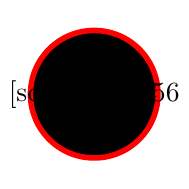
\begin{tikzpicture}[baseline={(current bounding box.center)}]
  \tikzset{pgfornamentstyle/.style={
            draw=Goldenrod,fill=Red,line width=1pt}}
  \node[fill=black,circle,draw=Red,line width=2pt,inner sep=-8pt]
    at (0,0) {\pgfornamenthan[scale=0.38]{56}};
\end{tikzpicture}
\end{tcblisting}

\begin{tcblisting}{title={简单的边框范例}}

\begin{tikzpicture}[x=1pt,y=1pt]
    \tikzset{every node/.append style={inner sep=0pt,color=茜色}}
    \node (nw) {\pgfornamenthan[scale=0.35]{1}};
    \node[anchor=north west,right=140bp of nw] (ne) {\pgfornamenthan[symmetry=v,scale=0.35]{1}};
    \node[anchor=north west,below=0pt of nw] (sw) {\pgfornamenthan[symmetry=h,scale=0.35]{1}};
    \node[anchor=north east,below=0pt of ne] (se) {\pgfornamenthan[symmetry=c,scale=0.35]{1}};

    %% 用 pgfornmanet 自带的 \draw (A) to[ornamenthan=19] (B) 机制的话会导致线条高度跟着变化!只好折衷用tikz的 xscale 来实现加长了。\pgfornamenthan 本身的 scale 则要确保和角点的 scale 一致。
    \node[anchor=south west,xscale=2] at (sw.south east) {\pgfornamenthan[scale=0.35]{29}};

    %% 另外一种方法是用 decorations,同样需要注意一下各种长度参数
    \begin{scope}[decoration={markings,
      mark=between positions 0 and 0.75 step 70bp with
        { \node[transform shape,anchor=north west]{\pgfornamenthan[scale=0.35]{29}};}
      }]
      \draw[decorate] (nw.north east) -- (ne.north west);
    \end{scope}

  \node[font=\kaishu,align=center,xshift=70,text=black] at (nw.south east)
     {给我一片海棠红啊海棠红\\血一样的海棠红\\
     沸血的烧痛是乡愁的烧痛\\给我一片海棠红啊海棠红};
\end{tikzpicture}
\end{tcblisting}

\begin{tcblisting}{title={另一个简单的边框范例}}
\begin{tikzpicture}
  \tikzset{every node/.append style={铜绿,inner sep=0pt}}
  \node (nw) {\pgfornamenthan[scale=0.25]{12}};
  \node[right=50bp of nw] (ne) {\pgfornamenthan[scale=0.25,symmetry=v]{12}};
  \node[below=50bp of nw] (sw) {\pgfornamenthan[scale=0.25,symmetry=h]{12}};
  \node[below=50bp of ne] (se) {\pgfornamenthan[scale=0.25,symmetry=c]{12}};
  % 每个部件原宽度为200bp,因此绘画时如果以bp作为单位,会比较容易计算xscale的值。这里 scale=0.25 则部件有效宽度为50bp,刚好是两个角点符号之间的距离,因此不需要再设 xscale。
  \node[anchor=north west] at (nw.north east) {\pgfornamenthan[scale=0.25]{32}};
  \node[anchor=south west] at (sw.south east) {\pgfornamenthan[scale=0.25]{32}};
  \node[anchor=south west,rotate=-90] at (nw.south west) {\pgfornamenthan[scale=0.25]{32}};
  \node[anchor=south east,rotate=90] at (ne.south east) {\pgfornamenthan[scale=0.25]{32}};

\node[anchor=center,靛蓝,shift={(25bp,-25bp)}] at (nw.south east) {\pgfornamenthan[scale=0.5]{57}};
\end{tikzpicture}
\end{tcblisting}


\begin{tcblisting}{title=有些部件衔接可能需要手动\texttt{shift}}
  \begin{tikzpicture}\tikzset{every node/.append style={赤金,inner sep=0pt}}
    \node (nw) {\pgfornamenthan[scale=0.2]{23}};
    \node[right=53bp of nw] (ne) {\pgfornamenthan[scale=0.2,symmetry=v]{23}};
    \node[anchor=north west,xshift=2bp] at (nw.north east) {\pgfornamenthan[scale=0.2]{41}};
    \node[anchor=north east,xshift=-2bp] at (ne.north west) {\pgfornamenthan[scale=0.2,symmetry=v]{41}};
  \end{tikzpicture}
\end{tcblisting}

\begin{tcblisting}{listing only,title={框着整个页面的代码。很适合拿来设计奖状证书的有木有!}}
  \newbox{\fortyseven}
  \savebox{\fortyseven}{\pgfornamenthan[scale=0.2,color=鸭卵青]{47}}
  \tikzset{every node/.append style={inner sep=0pt,鸭卵青}}
  \begin{tikzpicture}[overlay,remember picture]
  \node[anchor=north west,shift={(14.5pt,-14.5pt)}] at (current page.north west)
    (nw) {\pgfornamenthan[scale=0.2]{25}};
  \node[anchor=north east,shift={(-14.5pt,-14.5pt)}] at (current page.north east)
    (ne) {\pgfornamenthan[scale=0.2,symmetry=v]{25}};
  \node[anchor=south west,shift={(14.5pt,14.5pt)}] at (current page.south west)
    (sw) {\pgfornamenthan[scale=0.2,symmetry=h]{25}};
  \node[anchor=south east,shift={(-14.5pt,14.5pt)}] at (current page.south east)
    (se) {\pgfornamenthan[scale=0.2,symmetry=c]{25}};
  %
  \begin{scope}[start chain,node distance=0pt]
  \node[anchor=north west,on chain] at (nw.north east) {\usebox{\fortyseven}};
  \foreach \i in {1,...,15} {
    \node[on chain]{\usebox{\fortyseven}};
  }
  \end{scope}
  %
  \begin{scope}[start chain,node distance=0pt]
  \node[anchor=south west,on chain] at (sw.south east) {\usebox{\fortyseven}};
  \foreach \i in {1,...,6} \node[on chain]{\usebox{\fortyseven}};
  \end{scope}
  %
  \begin{scope}[start chain=going left,node distance=0pt]
  \node[anchor=south east,on chain] at (se.south west) {\usebox{\fortyseven}};
  \foreach \i in {1,...,6} \node[on chain]{\usebox{\fortyseven}};
  \end{scope}
  %
  % 垂直的话 chains 比较不好控制,我懒得折腾了,直接用 \foreach。
  % 自己算一下, (47) 长度 155. 那么 scale = 0.2 的话……
  \foreach \i in {0,...,21}
    \node[anchor=south west,rotate=-90,shift={($\i*(31bp,0)$)}] at (nw.south west)
      {\usebox{\fortyseven}};
  %
  \foreach \i in {0,...,21}
    \node[anchor=south east,rotate=90,shift={($\i*(-31bp,0)$)}] at (ne.south east)
      {\usebox{\fortyseven}};
  %
  %% 严格来说应该放在 \fancyfoot 吧,算了一样啦
  \node[yshift=32pt,铜绿] at (current page.south) {\pgfornamenthan[scale=0.1]{51}};
  \node[yshift=32pt,text=black] at (current page.south) {\large\thepage};
  %
  \end{tikzpicture}
\end{tcblisting}

\part{纹样列表}

以下部件的原宽度、原高度皆以1bp为单元。


\setlength{\parindent}{0pt}\raggedright

\section{角点符号}

\subsection{接单线的角点符号}

有实心线型与对应的空心线型两种。以下皆同。

\bigskip


\foreach \n in {1,...,8}{%
  \begin{tikzpicture}
    \fill[牙色](-1cm,-1cm) rectangle (1cm,1cm);
    \node[inner sep=0pt] (element) {\pgfornamenthan[color=茜色,width=1.8cm]{\n}};
    \node[inner sep=0pt,font=\footnotesize\bfseries\sffamily,color=紫檀] at (0.8cm,-0.8cm) {\n};
    \node[anchor=west,text width=4em,font=\footnotesize] at (1.1cm,0) {\getpgfornamenthanDim{\n}};
    \draw[color=牙色] (1cm,-1cm) rectangle (2.8cm,1cm);
  \end{tikzpicture}\space\space
}

\subsection{接双线的角点符号}

\foreach \n in {9,...,14}{%
  \begin{tikzpicture}
    \fill[牙色](-1cm,-1cm) rectangle (1cm,1cm);
    \node[inner sep=0pt] (element) {\pgfornamenthan[color=茜色,width=1.8cm]{\n}};
    \node[inner sep=0pt,font=\footnotesize\bfseries\sffamily,color=紫檀] at (0.8cm,-0.8cm) {\n};
    \node[anchor=west,text width=4em,font=\footnotesize] at (1.1cm,0) {\getpgfornamenthanDim{\n}};
    \draw[color=牙色] (1cm,-1cm) rectangle (2.8cm,1cm);
  \end{tikzpicture}\space\space
}


\subsection{简单角点符号}

和其他角点符号配合,在一条对角线上使用其他角点符号,另一条对角 线上使用简单角点符号。

\bigskip

\foreach \n in {15,...,18}{%
  \begin{tikzpicture}
    \fill[牙色](-1cm,-1cm) rectangle (1cm,1cm);
    \node[inner sep=0pt] (element) {\pgfornamenthan[color=茜色,width=1.8cm]{\n}};
    \node[inner sep=0pt,font=\footnotesize\bfseries\sffamily,color=紫檀] at (0.8cm,-0.8cm) {\n};
    \node[anchor=west,text width=4em,font=\footnotesize] at (1.1cm,0) {\getpgfornamenthanDim{\n}};
    \draw[color=牙色] (1cm,-1cm) rectangle (2.8cm,1cm);
  \end{tikzpicture}\space\space
}

\subsection{回纹的角点符号}

和连续的回纹配合。

\bigskip

\foreach \n in {19,...,22}{%
  \begin{tikzpicture}
    \fill[牙色](-1cm,-1cm) rectangle (1cm,1cm);
    \node[inner sep=0pt] (element) {\pgfornamenthan[color=茜色,width=1.8cm]{\n}};
    \node[inner sep=0pt,font=\footnotesize\bfseries\sffamily,color=紫檀] at (0.8cm,-0.8cm) {\n};
    \node[anchor=west,text width=4em,font=\footnotesize] at (1.1cm,0) {\getpgfornamenthanDim{\n}};
    \draw[color=牙色] (1cm,-1cm) rectangle (2.8cm,1cm);
  \end{tikzpicture}\space\space
}

\bigskip\bigskip

和离散的回纹配合。

\bigskip

\foreach \n in {23,...,28}{%
  \begin{tikzpicture}
    \fill[牙色](-1cm,-1cm) rectangle (1cm,1cm);
    \node[inner sep=0pt] (element) {\pgfornamenthan[color=茜色,width=1.8cm]{\n}};
    \node[inner sep=0pt,font=\footnotesize\bfseries\sffamily,color=紫檀] at (0.8cm,-0.8cm) {\n};
    \node[anchor=west,text width=4em,font=\footnotesize] at (1.1cm,0) {\getpgfornamenthanDim{\n}};
    \draw[color=牙色] (1cm,-1cm) rectangle (2.8cm,1cm);
  \end{tikzpicture}\space\space
}


\section{线型单元}

\subsection{单线、双线直线}

\foreach \n in {29,...,32}{%
  \begin{tikzpicture}
    \fill[牙色](-1cm,-1cm) rectangle (1cm,1cm);
    \node[inner sep=0pt] (element) {\pgfornamenthan[color=茜色,width=1.8cm]{\n}};
    \node[inner sep=0pt,font=\footnotesize\bfseries\sffamily,color=紫檀] at (0.8cm,-0.8cm) {\n};
    \node[anchor=west,text width=4em,font=\footnotesize] at (1.1cm,0) {\getpgfornamenthanDim{\n}};
    \draw[color=牙色] (1cm,-1cm) rectangle (2.8cm,1cm);
  \end{tikzpicture}\space\space
}

\subsection{回字纹}

\subsubsection{连续}

\foreach \n in {33,...,36}{%
  \begin{tikzpicture}
    \fill[牙色](-1cm,-1.1cm) rectangle (1cm,0.9cm);
    \node[inner sep=0pt] (element) {\pgfornamenthan[color=茜色,height=0.6cm]{\n}};
    \node[inner sep=0pt,font=\footnotesize\bfseries\sffamily,color=紫檀] at (0.8cm,-0.9cm) {\n};
    \node[anchor=west,text width=4em,font=\footnotesize] at (1.1cm,0) {\getpgfornamenthanDim{\n}};
    \draw[color=牙色] (1cm,-1.1cm) rectangle (2.8cm,0.9cm);
  \end{tikzpicture}\space\space
}%
\foreach \n in {37,...,40}{%
  \begin{tikzpicture}
    \fill[牙色](-1cm,-1.1cm) rectangle (1cm,0.9cm);
    \node[inner sep=0pt] (element) {\pgfornamenthan[color=茜色,height=1.1cm]{\n}};
    \node[inner sep=0pt,font=\footnotesize\bfseries\sffamily,color=紫檀] at (0.8cm,-0.9cm) {\n};
    \node[anchor=west,text width=4em,font=\footnotesize] at (1.1cm,0) {\getpgfornamenthanDim{\n}};
    \draw[color=牙色] (1cm,-1.1cm) rectangle (2.8cm,0.9cm);
  \end{tikzpicture}\space\space
}

\subsubsection{离散}

\foreach \n in {41,...,44}{%
  \begin{tikzpicture}
    \fill[牙色](-1cm,-1.1cm) rectangle (1cm,0.9cm);
    \node[inner sep=0pt] (element) {\pgfornamenthan[color=茜色,height=0.6cm]{\n}};
    \node[inner sep=0pt,font=\footnotesize\bfseries\sffamily,color=紫檀] at (0.8cm,-0.9cm) {\n};
    \node[anchor=west,text width=4em,font=\footnotesize] at (1.1cm,0) {\getpgfornamenthanDim{\n}};
    \draw[color=牙色] (1cm,-1.1cm) rectangle (2.8cm,0.9cm);
  \end{tikzpicture}\space\space
}

\subsubsection{离散连接}

\foreach \n in {45,...,48}{%
  \begin{tikzpicture}
    \fill[牙色](-1cm,-1.1cm) rectangle (1cm,0.9cm);
    \node[inner sep=0pt] (element) {\pgfornamenthan[color=茜色,height=0.6cm]{\n}};
    \node[inner sep=0pt,font=\footnotesize\bfseries\sffamily,color=紫檀] at (0.8cm,-0.9cm) {\n};
    \node[anchor=west,text width=4em,font=\footnotesize] at (1.1cm,0) {\getpgfornamenthanDim{\n}};
    \draw[color=牙色] (1cm,-1.1cm) rectangle (2.8cm,0.9cm);
  \end{tikzpicture}\space\space
}

\subsubsection{圆周排布的回纹}
\foreach \n in {49,...,54}{%
  \begin{tikzpicture}
    \fill[牙色](-1.5cm,-1.5cm) rectangle (1.5cm,1.5cm);
    \node[inner sep=0pt] (element) {\pgfornamenthan[color=茜色,width=2.8cm]{\n}};
    \node[inner sep=0pt,font=\footnotesize\bfseries\sffamily,color=紫檀] at (0,0) {\n};
    \node[anchor=west,text width=4em,font=\footnotesize] at (1.6cm,0) {\getpgfornamenthanDim{\n}};
    \draw[color=牙色] (1.5cm,-1.5cm) rectangle (3.5cm,1.5cm);
  \end{tikzpicture}\space\space
}

\section{吉祥纹路}

\subsection{福字纹}

\foreach \n in {55}{%
  \begin{tikzpicture}
    \fill[牙色](-1cm,-1cm) rectangle (1cm,1cm);
    \node[inner sep=0pt] (element) {\pgfornamenthan[color=茜色,width=1.8cm]{\n}};
    \node[inner sep=0pt,font=\footnotesize\bfseries\sffamily,color=紫檀] at (0.8cm,-0.8cm) {\n};
    \node[anchor=west,text width=4em,font=\footnotesize] at (1.1cm,0) {\getpgfornamenthanDim{\n}};
    \draw[color=牙色] (1cm,-1cm) rectangle (2.8cm,1cm);
  \end{tikzpicture}\space\space
}

\subsection{寿字纹}

\foreach \n in {56,57}{%
  \begin{tikzpicture}
    \fill[牙色](-1cm,-1cm) rectangle (1cm,1cm);
    \node[inner sep=0pt] (element) {\pgfornamenthan[color=茜色,width=1.8cm]{\n}};
    \node[inner sep=0pt,font=\footnotesize\bfseries\sffamily,color=紫檀] at (0.8cm,-0.8cm) {\n};
    \node[anchor=west,text width=4em,font=\footnotesize] at (1.1cm,0) {\getpgfornamenthanDim{\n}};
    \draw[color=牙色] (1cm,-1cm) rectangle (2.8cm,1cm);
  \end{tikzpicture}\space\space
}

\section{云纹}

\subsection{对称符号}

\foreach \n in {58,...,61}{%
\begin{tikzpicture}
  \fill[牙色](-1.5cm,-1cm) rectangle (1.5cm,1cm);
  \node[inner sep=0pt] (element) {\pgfornamenthan[color=茜色,width=2.8cm]{\n}};
  \node[inner sep=0pt,font=\footnotesize\bfseries\sffamily,color=紫檀] at (1.3cm,-0.8cm) {\n};
  \node[anchor=west,text width=4em,font=\footnotesize] at (1.6cm,0) {\getpgfornamenthanDim{\n}};
  \draw[color=牙色] (1.5cm,-1cm) rectangle (3.5cm,1cm);
\end{tikzpicture}\space\space
}


\subsection{左右侧符号}

\foreach \n in {62,...,71}{%
  \begin{tikzpicture}
    \fill[牙色](-1cm,-1cm) rectangle (1cm,1cm);
    \node[inner sep=0pt] (element) {\pgfornamenthan[color=茜色,width=1.8cm]{\n}};
    \node[inner sep=0pt,font=\footnotesize\bfseries\sffamily,color=紫檀] at (0.8cm,-0.8cm) {\n};
    \node[anchor=west,text width=4em,font=\footnotesize] at (1.1cm,0) {\getpgfornamenthanDim{\n}};
    \draw[color=牙色] (1cm,-1cm) rectangle (2.8cm,1cm);
  \end{tikzpicture}\space\space
}


\subsection{角落符号}

\foreach \n in {72,...,75}{%
  \begin{tikzpicture}
    \fill[牙色](-1cm,-1cm) rectangle (1cm,1cm);
    \node[inner sep=0pt] (element) {\pgfornamenthan[color=茜色,width=1.8cm]{\n}};
    \node[inner sep=0pt,font=\footnotesize\bfseries\sffamily,color=紫檀] at (0.8cm,0.8cm) {\n};
    \node[anchor=west,text width=4em,font=\footnotesize] at (1.1cm,0) {\getpgfornamenthanDim{\n}};
    \draw[color=牙色] (1cm,-1cm) rectangle (2.8cm,1cm);
  \end{tikzpicture}\space\space
}

\subsection{连接线}

\foreach \n in {76,...,77}{%
  \begin{tikzpicture}
    \fill[牙色](-1cm,-1cm) rectangle (1cm,1cm);
    \node[inner sep=0pt] (element) {\pgfornamenthan[color=茜色,width=1cm]{\n}};
    \node[inner sep=0pt,font=\footnotesize\bfseries\sffamily,color=紫檀] at (0.8cm,-0.8cm) {\n};
    \node[anchor=west,text width=4em,font=\footnotesize] at (1.1cm,0) {\getpgfornamenthanDim{\n}};
    \draw[color=牙色] (1cm,-1cm) rectangle (2.8cm,1cm);
  \end{tikzpicture}\space\space
}

\vfill

\begin{center}
\begin{tikzpicture}
  \tikzset{every node/.append style={铜绿,inner sep=0pt,node distance=0pt}}
  \node (nw) {\pgfornamenthan[scale=0.2]{6}};
  \node[right=100bp of nw] (ne) {\pgfornamenthan[scale=0.2,symmetry=v]{16}};
  \node[below=-8bp of nw] (sw) {\pgfornamenthan[scale=0.2,symmetry=h]{16}};
  \node[below=-8bp of ne] (se) {\pgfornamenthan[scale=0.2,symmetry=c]{6}};
  \node[anchor=north west,xscale=2.5] at (nw.north east) {\pgfornamenthan[scale=0.2]{30}};
  \node[anchor=south west,xscale=2.5] at (sw.south east) {\pgfornamenthan[scale=0.2]{30}};
  \node[font=\kaishu\Large,text=black,shift={(50bp,4bp)}] at (nw.south east) {待续};
\end{tikzpicture}
\end{center}

\clearpage
\appendix
\ctexset{section/name={附录}}
\phantomsection\addcontentsline{toc}{part}{附录}

\section{传统中国颜色 \texttt{cncolours.sty}}

\begingroup
\centering
这是我比较早以前做的一个宏包了,色卡取自 \url{http://ylbook.com/cms/web/chuantongsecai/chuantongsecai.htm}。

\bigskip

\renewcommand{\baselinestretch}{2}
\newcommand\showcolour[1]{%
  \fcolorbox{乌黑}{#1}{\makebox[2em]{\phantom{M}}}~\makebox[5em][l]{#1}%
}

\showcolour{粉红}
\showcolour{妃色}
\showcolour{品红}
\showcolour{桃红}
\showcolour{海棠红}
\showcolour{石榴红}
\showcolour{樱桃色}
\showcolour{银红}
\showcolour{大红}
\showcolour{绛紫}
\showcolour{绯红}
\showcolour{胭脂}
\showcolour{朱红}
\showcolour{丹}
\showcolour{彤}
\showcolour{茜色}
\showcolour{火红}
\showcolour{赫赤}
\showcolour{嫣红}
\showcolour{洋红}
\showcolour{炎}
\showcolour{赤}
\showcolour{绾}
\showcolour{枣红}
\showcolour{檀}
\showcolour{殷红}
\showcolour{酡红}
\showcolour{酡颜}
\showcolour{鹅黄}
\showcolour{鸭黄}
\showcolour{樱草色}
\showcolour{杏黄}
\showcolour{杏红}
\showcolour{橘黄}
\showcolour{橙黄}
\showcolour{橘红}
\showcolour{姜黄}
\showcolour{缃色}
\showcolour{橙色}
\showcolour{茶色}
\showcolour{驼色}
\showcolour{昏黄}
\showcolour{栗色}
\showcolour{棕色}
\showcolour{棕绿}
\showcolour{棕黑}
\showcolour{棕红}
\showcolour{棕黄}
\showcolour{赭色}
\showcolour{琥珀}
\showcolour{褐色}
\showcolour{枯黄}
\showcolour{黄栌}
\showcolour{秋色}
\showcolour{秋香色}
\showcolour{嫩绿}
\showcolour{柳黄}
\showcolour{柳绿}
\showcolour{竹青}
\showcolour{葱黄}
\showcolour{葱绿}
\showcolour{葱青}
\showcolour{青葱}
\showcolour{油绿}
\showcolour{绿沉}
\showcolour{碧色}
\showcolour{碧绿}
\showcolour{青碧}
\showcolour{翡翠色}
\showcolour{草绿}
\showcolour{青色}
\showcolour{青翠}
\showcolour{青白}
\showcolour{鸭卵青}
\showcolour{蟹壳青}
\showcolour{鸦青}
\showcolour{绿色}
\showcolour{豆绿}
\showcolour{豆青}
\showcolour{石青}
\showcolour{玉色}
\showcolour{缥}
\showcolour{艾绿}
\showcolour{松柏绿}
\showcolour{松花绿}
\showcolour{松花色}
\showcolour{蓝}
\showcolour{靛青}
\showcolour{靛蓝}
\showcolour{碧蓝}
\showcolour{蔚蓝}
\showcolour{宝蓝}
\showcolour{蓝灰色}
\showcolour{藏青}
\showcolour{藏蓝}
\showcolour{黛}
\showcolour{黛绿}
\showcolour{黛蓝}
\showcolour{黛紫}
\showcolour{紫色}
\showcolour{紫酱}
\showcolour{酱紫}
\showcolour{紫檀}
\showcolour{绀青}
\showcolour{紫棠}
\showcolour{青莲}
\showcolour{群青}
\showcolour{雪青}
\showcolour{丁香色}
\showcolour{藕色}
\showcolour{藕荷色}
\showcolour{苍色}
\showcolour{苍黄}
\showcolour{苍青}
\showcolour{苍黑}
\showcolour{苍白}
\showcolour{水色}
\showcolour{水红}
\showcolour{水绿}
\showcolour{水蓝}
\showcolour{淡青}
\showcolour{湖蓝}
\showcolour{湖绿}
\showcolour{精白}
\showcolour{象牙白}
\showcolour{雪白}
\showcolour{月白}
\showcolour{缟}
\showcolour{素}
\showcolour{荼白}
\showcolour{霜色}
\showcolour{花白}
\showcolour{鱼肚白}
\showcolour{莹白}
\showcolour{灰色}
\showcolour{牙色}
\showcolour{铅白}
\showcolour{玄色}
\showcolour{玄青}
\showcolour{乌色}
\showcolour{乌黑}
\showcolour{漆黑}
\showcolour{墨色}
\showcolour{墨灰}
\showcolour{黑色}
\showcolour{缁色}
\showcolour{煤黑}
\showcolour{黧}
\showcolour{黎}
\showcolour{黝}
\showcolour{黝黑}
\showcolour{黯}
\showcolour{赤金}
\showcolour{金色}
\showcolour{银白}
\showcolour{铜绿}
\showcolour{乌金}
\showcolour{老银}

\endgroup

\clearpage

\section{萧山 Beamer 主题 Xiaoshan Beamer Theme \texttt{beamerthemeXiaoshan.sty}}

这个Beamer主题是以 \href{https://ctan.org/pkg/beamertheme-metropolis}{Metropolis} 为基础,用 \texttt{cncolours.sty} 调了一下颜色,加入少许汉风纹样。

\bigskip

\begin{tcblisting}{listing side comment,title={使用范例},pdf comment={XiaoShanSample.pdf}}
\documentclass{ctexbeamer}

\usetheme{Xiaoshan}

\author{林莲枝}
\title{萧山Beamer主题}
\subtitle{\texttt{pgfornament-han}附录福利}

\begin{document}

\begin{frame}
  \maketitle
\end{frame}

\section{简介}

\begin{frame}
  \frametitle{其实是 Metropolis 主题的魔改}
  \begin{itemize}
    \item 改了颜色(用了 \texttt{cncolours.sty})
    \item 加入 \texttt{pgfornament-han} 汉风纹样元素
  \end{itemize}
\end{frame}
......
\end{document}
\end{tcblisting}

\end{document}
